\documentclass{article}
\usepackage[utf8]{inputenc}
\usepackage[english]{babel}
\usepackage{graphicx}
\usepackage{float}

\begin{document}
\title{A Comparison of Dining Philosopher Solutions}
\author{Chris Dellomes\\
Professor: Carol LeDoux\\
CMSI 387: Operating Systems\\
	Loyola Marymount University}

\date{April 18, 2016}

\maketitle

\begin{center}
\begin{abstract}
This study is in response to the significance of the dining philosopher's problem in the field of operating systems. Synchronization and deadlock are important factors in the operating system development, which are simluated within the parameters of the problem. This paper presents comparative evaluations of three different solutions: Dijkstra's original solution, an arbitrator solution, and Chandy and Misra's cleanliness solution. Overall, the solution presented by Chandy andd Misra is the most effective of the three based on its scalability and efficiency.
\end{abstract}
\end{center}

\thispagestyle{empty}

\clearpage

\setcounter{page}{1}

\section{Introduction} The dining philosopher's problem is a significant point of discussion in the field of operating systems. It is a direct derivation of general issue of concurrent resource allocation, and thus the development of an efficient solution is a source of research and debate. The problem is defined as five philosophers at a table with five chopsticks between them to be used to eat. Each philosopher picks up each chopstick individually and is either in the process of eating or wating to eatThis paper will present a comparison of three distinct solutions and their overall effectiveness based on the criteria established by the problem's parameters. The problem was first proposed by Edsger Dijkstra, who developed an accompanying resource hierarchy algorithm for allocating the chopsticks amongst the philosophers. An alterante solution is to introduce an arbitrator entity, which moderates resource requests. In an attempt to improve upon previous solutions, Dr. Kanianthra Chandy and Dr. Jayadev Misra developed a solution in which resources are labeled as clean or dirty and are passed between requesting philosophers. Based on its scalability and lack of overhead, the solution developed by Chandy and Misra is the most effective and applicable to modern day operating systems.

\section{Background} The dining philosopher problem was originally invented by Dr. Edsger Dijkstra in 1965 as an exercise for his students. The problem was created to represent deadlock and starvation related problems in synchronization andd concurrent algorithm design. The problem was initially defined as five philosophers, who at anytime are either waiting or eating with five chopsticks between them. When a philosopher tries to eat, the philosopher picks up two chopsticks one at a time. The problem asks for a way to ensure every philosopher has the chance to eat. The solution avoids deadlock, but is slow to perform. After making the problem, Dijkstra proposed an accompanying solution in which each chopstick is numbered and each philosopher picks up the lower numbered chopsticks first. Following Dijkstra's creation of the problem and his initial solution, another solution surfaced which involves a waiter that regulates when philosophers can eat. The philosophers must ask the waiter if they are allowed to eat, after which the waiter checks to see if there are enough chopsticks available to satisfy the request, which results in an instruction to either take the chopsticks and eat or to continue waiting. The solution avoids deadlock, but reduces concurrent performance. In 1984, Dr. Kanianthra Chandy and Dr. Jayadev Misra, professors at CalTech and UT Austin, respectively, cooperatively developed a solution which introduces a cleanliness traits to all chopsticks. The solution is scalable to an arbitrarily large number of philosophers and chopsticks and prevents deadlock as well as starvation. As time has progressed, so have the effectiveness of solutions.

\section{Problem Description} The dining philosopher problem is defined as five philosophers all sitting together at a round table with five chopsticks for all of them to use. Each philosopher is either eating or waiting to eat. In order to eat, a philosopher must pick up and use the chopsticks to the immediate right and left one at a time. After eating, the philosopher puts down each chopstick one at a time. The philosophers are also not allowed to speak to each other. The goal of any solution is to ensure that every philosopher has a chance to eat.

\begin{figure}[H]
\begin{center}
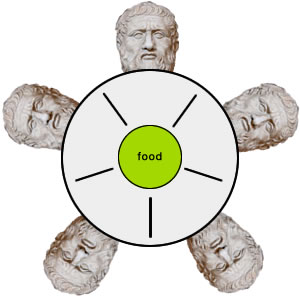
\includegraphics[width=0.2\textwidth]{diningphilosophers.jpg}
\caption{A visual representation of the dining philosopher's problem.}
\end{center}
\end{figure}

\section{Dijkstra's Solution} After creating and introducing the dining philosopher's problem to the field of computer science, Dijkstra presented his own solution based on establishing a hierarchy of resources. The philosophers and chopsticks are ordered with each philosopher and chopstick given a corresponding value. The philosophers are also made to always pick up lower numbered of their two nearby chopsticks first. For example, if each philosopher were to attempt to pick up their chopsticks at the same time, philosopher five would not be able to because chopstick 1 is already taken by philosopher 1. However, philosopher four would have both chopsticks four and five because he picked up chopstick four then five.

\begin{figure}[H]
\begin{center}
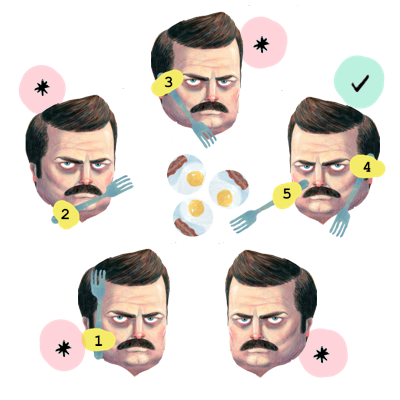
\includegraphics[width=0.3\textwidth]{resource.png}
\caption{A visual representation of the example using Dijkstra's resource allocation solution.}
\end{center}
\end{figure}

Dijkstra's solution ensures that there is no deadlock situation between philosophers trying to eat. Since deadlock is the primary focus of the dining philosopher's problem, Dijkstra ensures that ``the solution as presented is free from the danger of deadlock, as it should be.''. However, the solution lacks real world applicability due to the fact that ``it contains possibility of a particular philosopher being starved to death by a conspiration of his two neighbours'' [Dijkstra 1972]. Although a deadlock situation is impossible, starvation is still a possibility using Dijkstra's solution. Another weak point of the solution is its need to know the required resources beforehand. For example, if a process required resources three and five, then additionally requested resource two, then it must drop resources three and five before taking all three resources. Since the resource needs of a process are not always completely known beforehand, this weakness reduces the overall efficiency of the algorithm. Due to the possibility of starvation and lack of real world applicability, Dijkstra's original solution is an inefficient and barely acceptable solution to the dining philosopher's problem. Even Dijkstra found the solution to be ``so ugly, because the ordering of the semaphores is so arbitrary. I can only accept it, provided the total time spent in the excluded actions is such a negligable fraction of real time that actual delay in a P-operation is, indeed, extremely rare and always short,'' [Dijkstra]

\section{Arbitrator Solution} Along with Dijkstra's algorithm, another solution is to implement an arbitrator through which processes request the necessary resources. With the lack of preemption by themselves, the philosophers have the chance to put each other in deadlock by holding onto a single chopstick indefinitely. A way of eliminating deadlock opportunities is to introduce an arbitrator, implemented using a mutex, which regulates when a philosopher is able to pick up chopsticks to eat. Philosophers must request the arbitrator for both chopsticks to eat, at which point the arbitrator would determine if the necessary resources are available for distribution. Once a philosopher is finished eating, the chopsticks are returned to the arbitrator for use by other philosophers.

The solution is effective in eliminating possible deadlock by ensuring philosophers only acquire chopsticks once there are enough to ensure the philosopher eats. Starvation is also eliminated because each philosopher is ensured to have its request to eat fulfilled by the arbitrator's regulation of resources. However, the algorithm suffers from reduced parallelism. With each philosopher having to request resources from the arbitrator and return them one at a time, the number of events performed concurrently is reduced. Since concurrency is a primary focus of the dining philosopher's problem, the reduction in synchronized efficiency is a major drawback of the arbitrator solution.

\section{Chandy and Misra Solution} Professors Chandy and Misra developed their own solution to the dining philosopher's problem and published a paper on it in 1984. The solution is based around introducing a concept of cleanliness to the resources. The philosophers are ordered with each philosopher given an accompanying value. Chopsticks can either be clean or dirty and are all initially dirty. Every time a philosopher wants to eat and requires a chopstick, a request must be sent to the appropriate neighboring philosopher. Once a philosopher receives a request message, the philosopher retains the chopstick if it is clean, but cleans then passes it off if it is dirty. Once a philosopher eats, the chopsticks he used become dirty, which are then cleaned and passed on if they were previously requested by another philosopher.

\begin{figure}[H]
\begin{center}
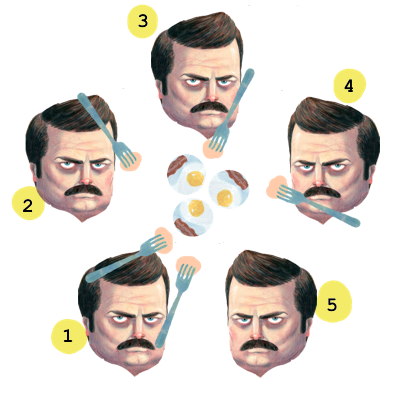
\includegraphics[width=0.3\textwidth]{clean.png}
\caption{A visual representation of Chandry and Misra's cleanliness based solution. The forks are all initially dirty.}
\end{center}
\end{figure}

The solution presented by Chandry and Misra ensure that there is no possibility of deadlock between philosophers. In their solution's presentation paper, Chandry and Misra demonstrate that ``The algorithm ensures that if processes u and v are in conflict, and u hasprecedence over v in the precedence graph, then the conflict resolution rule will,eventually, cause conflicts to be resolved in u's favor,'' which results in a process always being allowed to finish, thus preventing deadlock [Chandry and Misra 1984]. Additionally, no central authority is required to ensure protection from deadlock or starvation circumstances, eliminating overhead. Also, the solution scales to an arbitrarily large number \emph{n} amount of philosophers and chopsticks. Along with preventing a deadlock situation, the algorithm also solves the starvation issue by giving preference to starving processes through the use of the cleanliness attribute. However, the solution uses message passing in order for philosophers to request chopsticks from each other, which violates the predefined rule of not allowing the philosophers to communicate with one another. Although it breaks one of the original rules, the cleanliness based approach prevents both deadlock and starvation, scales efficiently to arbitrarily large values, and requires no overhead. Thus, the solution is the most efficient and applicable to real world concurrent system design.

\section{Conclusion} Between the different proposed solutions, the one developed by Chandry and Misra is the most efficient due to its preventative nature, scalability, and lack of required overhead. Though the original creator of the problem, Dijkstra's original algorithm fails to scale and prevent starvation, making it ineffective solution. On the other hand, the arbitrator solution successfully prevents deadlock and starvation, but at the cost of concurrent performance, efficiency, and required overhead. Based on its fulfillment of the primary requirements of the original problem and real world applicabillity, the cleanliness based solution created by Chandy and Misra is the most effective solution.

\begin{thebibliography}{100}

\bibitem{Sequential} ``Hierarchical Ordering of Sequential Processes", \emph{Acta-Informatica} http://link.springer.com/article/10.1007/BF00289519
\bibitem{Chandy} ``The Drinking Philosophers Problem", \emph{ACM Transactions on Programming Languages and Systems} https://www.cs.utexas.edu/users/misra/scannedPdf.dir/DrinkingPhil.pdf
\bibitem{Dijkstra} ``EWD625". \emph{Plataanstrat} https://www.cs.utexas.edu/users/EWD/ewd06xx/EWD625.PDF


\end{thebibliography}

\end{document}